\section{Úvod}
Následující dokument popisuje způsob implementace kompilátoru z~jazyka IFJ17 do mezikódu
IFJcode17 ve variantě 2. Jedná se o~projekt,
který byl vyprácován podle zadání do předmětů IAL a IFJ na Fakultě
informačních technologí Vysokého učení technického v~Brně.

Dokumentace popisuje způsob řešení, dekompozici překladače na jednotlivé části,
způsob práce v~týmu a popis použitých algoritmů a datových struktur.

\section{Teoretický rozbor projektu}
Naším úkolem bylo implementovat překladač jazyka IFJ17 (který je podmnožinou jazyka známého jako FREEBASIC) do mezikódu IFJcode17. Program čte zdrojový kód ze standardního vstupu a v~případě překladu bez chyby generuje cílový kód. V~případě chyby je navrácen odpovídající chybový kód a vytisknuta informace o~typu chyby.
Varianta 2 specifikuje zadání na užití tabulky s~rozptýlenými položkami při implementaci tabulky symbolů.

Pro běh překladače byl použit tzv. Syntaxí řízený překlad, což předurčuje syntaktický analyzátor k~získávání vstupních terminálů, spouštění sémantických kontrol a řízení konstrukce kódu. Optimalizátor poté pracuje mimo hlavní zpracování, je spuštěn po syntaktické analýze.

\begin{itemize}
    \item Lexikální analyzátor
    \item Syntaktický analyzátor
    \item Sémantický analyzátor,
    \item Generáto cílového kódu
    \item Optimalizátor kódu
\end{itemize}

Jelikož výstupem překladu je jistá forma mezikódu, používáme metodu generování tohoto kódu přímo ze syntaktické
analýzy bez generování abstraktního syntaktického stromu nebo zásobníkového kódu.

Propojení jednotlivých komponent naznačuje následující schéma.
\vspace*{4px}
\begin{figure}[htbp]
\centering
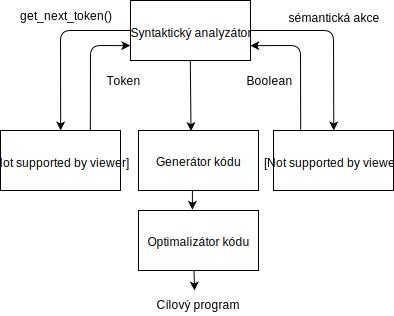
\includegraphics[width=0.65\textwidth, angle=0]{src/assets/structure.pdf}
\end{figure}